%%%%%%%%%%%%%%%%%%%%%%%%%%%%%%%%%%%%%%%%%%%%%%%%%%%%%%%%%%%%%%%%%%%%%%
\documentclass[12pt,twoside]{article}
\usepackage{weiiszablon}
\usepackage{float}

\type{Projekt}
\subject{Sztuczna Inteligencja}
\title{Temat: Zrealizować sieć neuronową uczoną algorytmem wstecznej propagacji błędu z przyśpieszeniem metodą adaptacyjnego współczynnika uczenia (trainbpa)
uczącą się rozpoznawania rodzaju wina}
\author{Szymon Kmieć}
\group{2EF-DI,	P2}

\begin{document}

% strona tytułowa
\maketitle

\blankpage

% spis treści
\tableofcontents

\clearpage
\blankpage


\section{Opis problemu}
Głównym celem projektu było zaprojektowanie oraz implementacja sieci neuronowej służącej do rozpoznawania gatunku wina. Do tego celu użyto własnej implementacji sieci neuronowej w języku Python 3.10.5 uczonej algorytmem wstecznej propagacji błędu. Jako metodę przyśpieszenia uczenia użyto adaptacyjnego współczynnika uczenia. W ramach projektu zbadano wpływ następujących parametrów na szybkość uczenia się sieci: 

%Głównym celem projektu było stworzenie algorytmu oraz nauczenie sieci neuronowej diagnozowania chorób na podstawie badań próbek tkanek z piersi. Została w tym celu stworzona sieć neuronowa uczona algorytmem wstecznej propagacji błędu. Jako metodę przyśpieszenia uczenia zastosowano adaptacyjny współczynnik uczenia. W ramach projektu zbadano wpływ parametrów na szybkość uczenia sieci:
\begin{itemize}
\item S1 - liczba neuronów w pierwszej warstwie sieci
\item S2 - liczba neuronów w drugiej warstwie sieci
\item lr - współczynnik uczenia sieci
\item er - współczynnik maksymalnego dopuszczalnego przyrostu błędu
\item lr\textsubscript{dec} - modyfikator współczynnika uczenia w przypadku przekroczeniu maksymalnego dopuszczalnego przyrostu błędu
\item lr\textsubscript{inc} - modyfikator współczynnika uczenia w przypadku spadku błędu
\end{itemize}

Opis problemu oraz wykorzystane w projekcie dane zostały przedstawione na stronie \cite{dane}

\clearpage

\section{Specyfikacja danych}
Dane pobrane z wspomnianej powyżej strony zawierały 178 wierszy danych, z których to każdy posiadał 14 atrybutów (w tym atrybut klasowy). Dane
są wynikiem analizy chemicznej win uprawianych w tym samym regionie Włoch,
ale pochodzących z trzech różnych odmian. Badany zestaw danych nie zawiera
niekompletnych rekordów, oraz wartości niepoprawnych. W zbiorze danych pierwszy
atrybut określa rodzaj wina - opisany liczbą całkowitą {1, 2, 3}, natomiast pozostałe
13 atrybutów to
\begin{itemize}
\item (Alcohol) - Procentowa zawartość alkoholu (wartość ciągła)
\item (Malic acid) - Procentowa zawartość kwasu jabłkowego (wartość ciągła)
\item (Ash) - Zawartość popiołu (wartość ciągła)
\item (Alkalinity of ash) - Zasadowość popiołu (wartość ciągła)
\item (Mg) - Zawartość magnezu (wartość ciągła)
\item (Total phenols) - Zawartość fenoli (wartość ciągła)
\item (Flavonoids) - Flawonoidy (wartość ciągła)
\item (Non Flavonoid phenols) - Fenole nieflawonoidowe (wartość ciągła)
\item (Proanthocyanins) - Proantocyjanidyny (wartość ciągła)
\item (Colour intensity) - Intensywność barwy (wartość ciągła)
\item (Hue) - Odcień (wartość ciągła)
\item (OD280/0D315) (wartość ciągła)
\item (Proline) - Prolina (wartość dyskretna)
\end{itemize}
\clearpage

\subsection{Normalizacja danych}
W celu usprawnienia procesu uczenia dane wejściowe zostały poddane normalizacji metodą \textit{min - max} określoną wzorem \cite{norm}:
\begin{equation}
f(x) = \frac{x - \min{(x)}}{\max{(x)} - \min{(x)}}
\end{equation}


Dzięki takiej normalizacji, możliwe jest dynamiczne normalizowanie danych wejściowych do zadanego zakresu. W przypadku tego projektu został zastosowany przedział normalizacyjny $ [0, 1]$.\\

\begin{lstlisting}[language=Python,caption=Algorytm normalizacji,label={Kod1}]
    for column in norm_data.columns:
        if column !=0:
            norm_data[column] = (norm_data[column] - norm_data[column].min()) / (norm_data[column].max() - norm_data[column].min())

\end{lstlisting}

Numery klas, stanowiące dane wyjściowe, zostały natomiast przekształcone przy pomocy kodowania 1 z N do postaci trójelementowego wektora, zawierającego wartość 1 na pozycji odpowiadającej danej klasie oraz wartości 0 na pozostałych pozycjach.



\clearpage
\section{Zagadnienia teoretyczne}
\subsection{Model sztucznego neuronu}
Sieć neuronową  tworzą pojedyncze neurony, które ułożone są w poszczególnych warstwach sieci. Neuron jest jednostką przetwarzającą informacje otrzymane na wejciu, oraz zwraca wynik przetwarzania w postaci wartości wyjściowej. 


Początkowo neuron miał co najmniej jedno wejście binarne i tylko jedno binarne wyjście. Wyjście było aktywowane, gdy osiągnięta została określona liczba wejść. W 1957 roku uczony Frank Rosenblatt zmodyfikował prosty sztuczny neuron binarny, tworząc w ten sposób perceptron, czyli jedną z najprostszych sieci neuronowych. Posiada on następującą charakterystykę \cite{mamczur}:
\begin{itemize}
\item Na wejściu i wyjściu mogą być dowolne liczby, nie tylko wartości binarne 
\item Połączenia węzłów mają określoną wagę
\item Wartość wyjściowa węzła składa się z dwóch części: sumy wartości z warstw poprzednich pomnożonej przez wagi oraz nałożonej na tą sumę funkcji aktywacji.
\end{itemize}

Model neuronu został przedstawiony na rysunku \ref{neuron}.

\begin{figure}[ht]
\label{neuron}
\centering
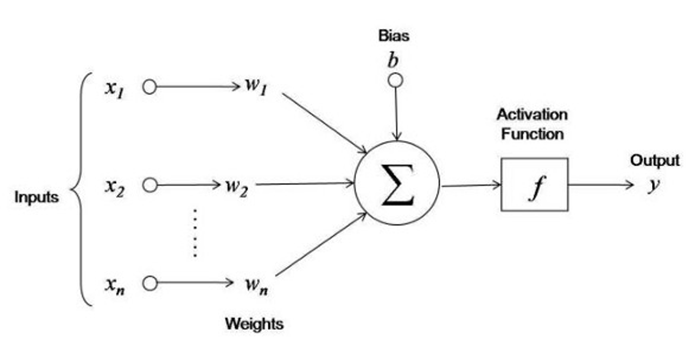
\includegraphics[width=14cm]{neuron.png}
\caption{Model neuronu}
\end{figure}

Ważona suma wejść wraz z przesunięciem nazywana jest łącznym pobudzeniem neuronu i określana wzorem:
\begin{equation}\label{pobudzenie}
z = \sum_{i=1}^{n}(x_i \cdot w_i) + b 
\end{equation}

Ogólny wzór na wartość wyjścia neuronu przedstawiono równaniem \ref{wyj-neu}

\begin{equation}\label{wyj-neu}
y = f \left(  \sum_{i=1}^{n}(x_i \cdot w_i) + b \right) = f(z)
\end{equation}
gdzie:
\begin{itemize}
\item $y$ - wyjście neuronu
\item $f$ - funkcja aktywacji
\item $n$ - ilość wejść
\item $x$ - wektor wejciowy
\item $w$ - wektor wag
\item $b$  - bias
\end{itemize}
Typy neuronów dzieli się ze względu na ich fukncję aktywacji. Najczęściej stosowanymi funkcjami aktywacji neuronu są funkcje sigmoidalne (\ref{siguni} oraz \ref{sigbi}) oraz liniowe (\ref{lin}).

Funkcja sigmoidalna unipolarna ma postać:
\begin{equation}\label{siguni}
f(x) = \frac{1}{1 + e^{-\beta x}}
\end{equation}

Funkcja sigmoidalna bipolarna:
\begin{equation}\label{sigbi}
f(x) = \frac{2}{1 + e^{-\beta x}} -1
\end{equation}

Funkcja liniowa:
\begin{equation}\label{lin}
f(x) = a \cdot x + b
\end{equation}

gdzie parametr $\beta$ najczęściej jest z przedziału $[0, 1]$.
\clearpage

\subsection{Sieć jednokierunkowa wielowarstwowa}

Sztuczną sieć neuronowa uzyskuje się łącząc ze sobą warstwy neuronów. Neurony nie łączą się ze sobą w obrębie tej samej warstwy lub z pominięciem warstw między nimi. Przykładowy model sieci wielowarstwowej pokazano na rysunku \ref{wielo}.

\begin{figure}[h]
\label{wielo}
\centering
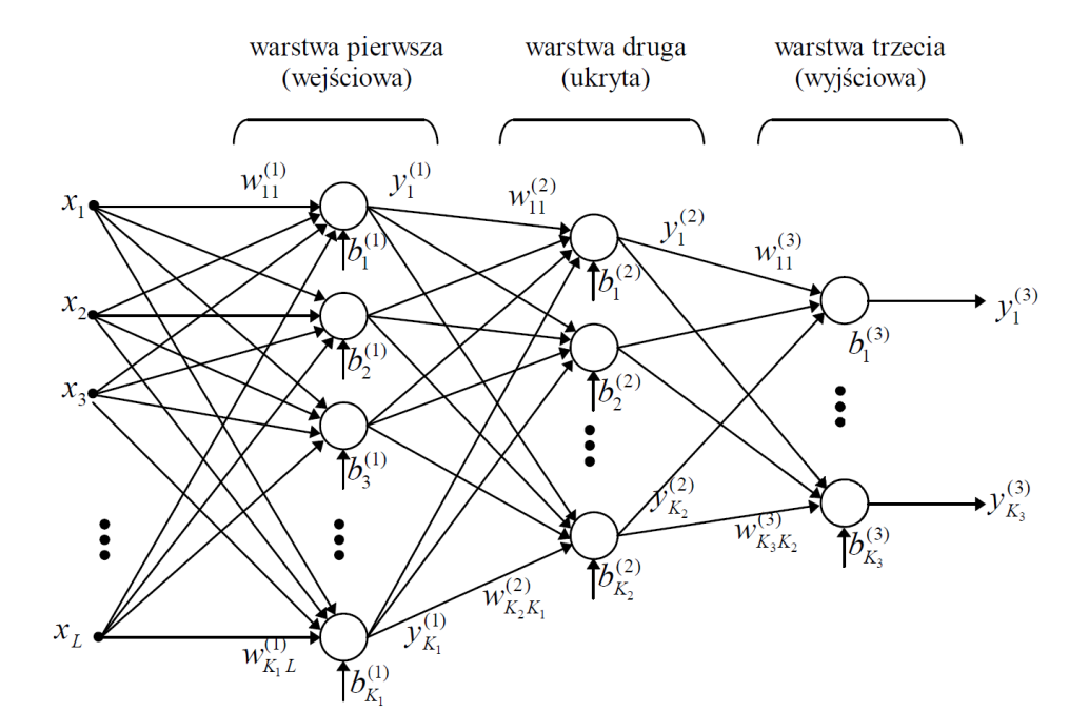
\includegraphics[width=14cm]{wielowarstwowa.png}
\caption{Sieć jednokierunkowa wielowarstwowa	[Źródło: \cite{zajdel1}]}
\end{figure}

Sieć taka ma zwykle strukturę obejmującą: 
\begin{itemize}
\item warstwę wejściową
\item jedną lub więcej warstw ukrytych (złożonych z neuronów sigmoidalnych)
\item warstwę wyjściową (złożoną z neuronów sigmoidalnych lub liniowych)
\end{itemize}

Charakterystyczną cechą dla warstwy wejściowej jest to, że nie bierze ona udziału w procesie uczenia, jej zadaniem zadaniem jest przekazanie wektora wejściowego sieci do warstw ukrytych, lub bezpośrednio do warstwy wyjściowej (w przypadku modelu sieci jednowarstwowej). Ilość warstw w sieci oraz ilość neuronów w warstwie są ściśle uzależnione od specyfiki problemu przed jakim zosataje postawiona sieć neuronowa.
\newpage
Każda warstwa sieci posiada:
\begin{itemize}
\item Macierz wag neuronów - $\textbf{w}$
\item Wektor przesunięć - $\textbf{b}$
\item Wektor sygnałów wyjściowych - $\textbf{y}$
\end{itemize}

Działanie poszczególnych warstw sieci opisane jest wzorami:
\begin{equation}\label{warstwy}
\begin{aligned}
y^{(1)} &= f^{(1)}(w^{(1)}x + b^{(1)})\\
y^{(2)} &= f^{(2)}(w^{(2)}y^{(1)} + b^{(2)})\\
y^{(3)} &= f^{(3)}(w^{(3)}y^{(2)} + b^{(3)})
\end{aligned}
\end{equation}

Zatem działanie całej trójwarstwowej sieci można zapisać jako:
\begin{equation}
y^{(3)} = f^{(3)}\left( w^{(3)} f^{(2)} \left( w^{(2)}f^{(1)} \left( w^{(1)}x + b^{(1)}\right) + b^{(2)} \right) + b^{(3)} \right)
\end{equation}
\\


\subsection{Algorytm wstecznej propagacji błędu}

Algorytm wstecznej propagacji błędu, nazywany również algorytmem największego spadku gradientu jest algorytmem dominującym wśród metod uczenia sieci jednokierunkowych. Działanie algorytmu sprowadza się do wyznaczenia gradientu funkcji celu dla każdego z neuronów sieci. 

Aby możliwe było zastosowanie algorytmu wstecznej propagacji błędu, wymagane jest, aby funkcje aktywacji neuronów były różniczkowalne. Pozwala to na wyznaczenie pochodnej błędu po danych wyjściowych. Dla każdej pary $(x, \hat{y})$ sieć popełnia błąd, który można zdefiniować następująco:

\begin{equation}
e = y - \hat{y}
\end{equation}

Celem uczenia sieci jest zminimalizowanie sumarycznego błędu kwadratowego, wyrażonego jako suma kwadratów błędów dla K neuronów w warstwie wyjściowej.

\begin{equation}\label{sredniokwad}
E = \frac{1}{2} \sum_{j=1}^{K} e_{j}^2
\end{equation}

W przypadku sieci z rysunku \ref{wielo} funkcja \ref{sredniokwad} po uwzględnieniu zależności \ref{warstwy} przyjmie postać:

\begin{equation}
\begin{aligned}
E =& \frac{1}{2} \sum_{i_{3}=1}^{K_{3}} e_{i_{3}}^2 = \frac{1}{2} \sum_{i_{3}=1}^{K_{3}}\left( y_{i_{3}}^{(3)} - \hat{y}_{i_{3}} \right)^2 =\\
 =& \frac{1}{2} \sum_{i_{3}=1}^{K_{3}} \left( f^{(3)}\left( \sum_{i_{2}=1}^{K_{2}} w_{i_{3}j_{2}}^{(3)}y_{i_{2}} + b_{i_{3}}^{(3)} \right) - \hat{y}_{i_{3}} \right)^2 =\\
=& \frac{1}{2} \sum_{i_{3}=1}^{K_{3}} \left( f^{(3)}\left( \sum_{i_{2}=1}^{K_{2}} w_{i_{3}j_{2}}^{(3)} f^{(2)}\left( \sum_{i_{1}=1}^{K_{1}} w_{i_{2}j_{1}}^{(2)} y_{i_{1}} + b_{i_{2}}^{(2)} \right) + b_{i_{3}}^{(3)} \right) - \hat{y}_{i_{3}} \right)^2 =\\
=& \frac{1}{2} \sum_{i_{3}=1}^{K_{3}} \left( f^{(3)}\left( \sum_{i_{2}=1}^{K_{2}} w_{i_{3}j_{2}}^{(3)} f^{(2)}\left( \sum_{i_{1}=1}^{K_{1}} w_{i_{2}j_{1}}^{(2)} f^{(1)}\left( \sum_{j=1}^{L} w_{i_{1}j}^{(1)} x_{j} + b_{i_{1}}^{(1)} \right) + b_{i_{2}}^{(2)} \right) + b_{i_{3}}^{(3)} \right) - \hat{y}_{i_{3}} \right)^2 
\end{aligned}
\end{equation}\\

Zminimalizowanie błędu \ref{sredniokwad} osiąga się poprzez zmianę biasów neuronów oraz wag ich połączeń. Kolejna wartość wagi połączenia jest wyznaczana na podstawie pochodnej cząstkowej błędu po wartości tejże wagi w obecnym cyklu nauczania. W podobny sposób wyznaczana jest również nowa wartość biasu dla każdego z neuronów. Otrzymaną pochodną mnoży się przez współczynnik uczenia $\eta$, który również może zmieniać się podczas procesu uczenia sieci. Zmiany poszczególnych wag obliczane są ze wzoru:\\
\begin{equation}
\Delta w_{ij} = - \eta \frac{\partial E}{\partial w_{ij}}
\end{equation}\\

Zatem wagę dla $k+1$ kroku otrzymać można w następujący sposób:\\
\begin{equation}
w_{ij}(k+1) = w_{ij}(k) - \eta \frac{\partial E}{\partial w_{ij}(k)}
\end{equation}\\

Obliczanie wag neuronów rozpoczyna się od warstwy wyjściowej:\\
\begin{equation}
\frac{\partial E}{\partial w_{i_{3}i_{2}}^{(3)}} = \frac{\partial E}{\partial f^{(3)}} \frac{\partial f^{(3)}\left( z_{i_{3}}^{(3)} \right)}{\partial z_{i_{3}}^{(3)}} \frac{\partial z_{i_{3}}^{(3)}}{\partial w_{i_{3}i_{2}}^{(3)}} = \left( y_{i_{3}} - \hat{y}_{i_{3}} \right) \frac{\partial f^{(3)}\left( z_{i_{3}}^{(3)} \right)}{\partial z_{i_{3}}^{(3)}} y_{i_{2}}^{(2)}
\end{equation}

Podobnie można obliczyć elementy gradientu względem wag warstwy ukrytej:\\
\begin{equation}
\begin{aligned}
&\frac{\partial E}{\partial w_{i_{2}i_{1}}^{(2)}} = \frac{\partial E}{\partial f^{(3)}} \frac{\partial f^{(3)}\left( z_{i_{3}}^{(3)} \right)}{\partial z_{i_{3}}^{(3)}} \frac{\partial z_{i_{3}}^{(3)}}{\partial f^{(2)}} \frac{\partial f^{(2)}\left( z_{i_{2}}^{(2)} \right)}{\partial z_{i_{2}}^{(2)}} \frac{\partial z_{i_{2}}^{(2)}}{\partial w_{i_{2}i_{1}}^{(2)}}  =\\
&= \sum_{i_{3}=1}^{K_3}\left( y_{i_{3}} - \hat{y}_{i_{3}} \right) \frac{\partial f^{(3)}\left( z_{i_{3}}^{(3)} \right)}{\partial z_{i_{3}}^{(3)}} w_{i_{3}i_{2}}^{(3)} \frac{\partial f^{(2)}\left( z_{i_{2}}^{(2)} \right)}{\partial z_{i_{2}}^{(2)}} y_{i_{1}}^{(1)}
\end{aligned}
\end{equation}\\

Oraz dla warstwy wejściowej:\\
\begin{equation}
\begin{aligned}
&\frac{\partial E}{\partial w_{i_{1}j}^{(1)}} = \frac{\partial E}{\partial f^{(3)}} \frac{\partial f^{(3)}\left( z_{i_{3}}^{(3)} \right)}{\partial z_{i_{3}}^{(3)}} \frac{\partial z_{i_{3}}^{(3)}}{\partial f^{(2)}} \frac{\partial f^{(2)}\left( z_{i_{2}}^{(2)} \right)}{\partial z_{i_{2}}^{(2)}} \frac{\partial z_{i_{2}}^{(2)}}{\partial f^{(1)}}  \frac{\partial f^{(1)}\left( z_{i_{1}}^{(1)} \right)}{\partial z_{i_{1}}^{(1)}} \frac{\partial z_{i_{1}}^{(1)}}{\partial w_{i_{1}j}^{(1)}}  =\\
&= \sum_{i_{3}=1}^{K_3}\left( y_{i_{3}} - \hat{y}_{i_{3}} \right) \frac{\partial f^{(3)}\left( z_{i_{3}}^{(3)} \right)}{\partial z_{i_{3}}^{(3)}} \sum_{i_{2}=1}^{K_2} w_{i_{3}i_{2}}^{(3)} \frac{\partial f^{(2)}\left( z_{i_{2}}^{(2)} \right)}{\partial z_{i_{2}}^{(2)}} w_{i_{2}i_{1}}^{(2)} \frac{\partial f^{(1)}\left( z_{i_{1}}^{(1)} \right)}{\partial z_{i_{1}}^{(1)}} x_j
\end{aligned}
\end{equation}
\\
\subsection{Adaptacyjny współczynik uczenia}

Algorytm wstecznej propagacji błędu jest dość czasochłonny. W celu przyśpieszenia procesu uczenia sieci korzysta się z metod pozwalających na jego przyśpieszenie. Jedną z nich jest metoda adaptacyjnej korekty współczynnika uczenia. Decyzję o zmianie podejmuje się na podstawie porównania błędu kwadratowego z jego wartością uzyskaną w poprzednim cyklu nauczania. Kolejną wartość $\eta$ otrzymuje się na podstawie następującej zależności:

\begin{equation}
\eta (t + 1) =
\left\{\begin{aligned}
\eta (t)  \xi_d  & \qquad gdy\ SSE(t) > er \cdot SSE(t - 1)\\
\eta (t)  \xi_i  & \qquad gdy\ SSE(t) < SSE(t - 1)\\
\eta (t)   & \qquad gdy\ SSE(t - 1) \leq SSE(t) \leq er \cdot SSE(t - 1)
\end{aligned}\right.
\end{equation}

gdzie:
\begin{itemize}
\item $er$ - dopuszczalna krotność przyrostu błędu
\item $\xi_d$ - współczynnik zmniejszania wartości współczynnika uczenia
\item $\xi_i$ - współczynnik zwiększania wartości współczynnika uczenia
\end{itemize}
\clearpage

\section{Implementacja sieci neuronowej}

Na potrzeby realizacji projektu zaimplementowano w języku Python program pozwalający na uczenie sieci neuronowej o dowolnej liczbie warstw algorytmem wstecznej propagacji błędu, wraz z przyspieszeniem metodą adaptacyjnego współczynnika uczenia na podstawie książki Michaela Nielsena \cite{nielsen}.  

Do implementacji wykorzystano język programowania Python 3.10.5, który jest językiem z natury wolnym, dlatego do obliczeń wykorzystano moduł \textit{numpy}. Moduł ten napisany jest w C, dzięki czemu obliczenia na macierzach będą wykonywane o wiele szybciej niż w zwykłym pythonie. Do kroswalidacji wykorzystano moduł \textit{sklearn}.

Kod źródłowy znajduje się na repozytorium GitHub \cite{github}

%Python jest z natury językiem wolnym. Dzieje się tak, ponieważ należy do grupy języków interpretowanych. Z racji tego, implementacja sieci w samym Pythonie byłaby nieefektywna. W związku z tym do obliczeń wykorzystano moduł \textit{numpy}. Biblioteka ta została napisana i skompilowana w języku C, dlatego wykonywanie obliczeń będzie znacznie przyspieszone. Do kroswalidacji użyto modułu \textit{sklearn}.

Program oferuje możliwość wyboru techniki aktualizacji wag:
\begin{itemize}
\item Wsadowa -  parametry neuronów aktualizowane są dopiero po wczytaniu do sieci całego zestawu danych uczących
\item Mini-batch -  Zbiór danych podzielony jest na podzbiory, aktualizacja parametrów sieci następuje po zaprezentowaniu całego podzbioru

\end{itemize}

\begin{lstlisting}[language=Python,caption=Implementacja sieci,label={Kod2}]
import random
import numpy as np

class Network(object):

    def __init__(self, sizes):
        np.random.seed(0x2f6eab9)
        self.num_layers = len(sizes)
        self.sizes = sizes
        self.biases = [np.random.randn(y, 1) for y in sizes[1:]]
        self.weights = [np.random.randn(y, x)
                        for x, y in zip(sizes[:-1], sizes[1:])]
        self.max_perf_inc = 1.04

    def __feedforward(self, a):
        for b, w in zip(self.biases, self.weights):
            a = self.__sigmoid(np.dot(w, a)+b)
        return a

    def __sse(self,_test_data):
        error=[pow(np.linalg.norm(self.__feedforward(x)-y),2) for (x,y) in _test_data]
        return 0.5*sum(error)    
 
    def train(self, training_data, test_data,epochs=1000,eta=0.1,error_goal=0.25,inc=1.05,dec=0.7,mini_batch_size=0,err_inc=1.04):
        self.max_perf_inc=err_inc
        if mini_batch_size==0: mini_batch_size=len(training_data)
        n_test = len(test_data)
        n = len(training_data)
        for j in range(epochs):
            random.shuffle(training_data)
            mini_batches = [training_data[k:k+mini_batch_size]
                    for k in range(0, n, mini_batch_size)]
            old_error=self.__sse(test_data)
            backup_weights = self.weights.copy()
            backup_biases = self.biases.copy()
            for mini_batch in mini_batches:
                self.__update_mini_batch(mini_batch, eta)
            new_error=self.__sse(test_data)
            if new_error < error_goal:
                test=self.__evaluate(test_data)
                test2=test/n_test*100
                print("Epoch {0}: {1:.2f}\%".format(j+1, test2))
                return [j+1, test2]
            elif new_error < old_error:
                eta *= inc
            elif new_error > old_error * self.max_perf_inc:
                self.weights = backup_weights
                self.biases = backup_biases
                eta *= dec
            if j==epochs-1:
                test=self.__evaluate(test_data)
                test2=test/n_test*100
                print("Epoch {0}: {1:.2f}\%".format(j+1, test2))
                return [j+1, test2]
    def __update_mini_batch(self, mini_batch, eta):
        nabla_b = [np.zeros(b.shape) for b in self.biases]
        nabla_w = [np.zeros(w.shape) for w in self.weights]
        for x, y in mini_batch:
            delta_nabla_b, delta_nabla_w = self.__backprop(x, y)
            nabla_b = [nb+dnb for nb, dnb in zip(nabla_b, delta_nabla_b)]
            nabla_w = [nw+dnw for nw, dnw in zip(nabla_w, delta_nabla_w)]
        self.weights = [w-(eta/2)*nw
                        for w, nw in zip(self.weights, nabla_w)]
        self.biases = [b-(eta/2)*nb
                       for b, nb in zip(self.biases, nabla_b)]

    def __backprop(self, x, y):
        nabla_b = [np.zeros(b.shape) for b in self.biases]
        nabla_w = [np.zeros(w.shape) for w in self.weights]
        # feedforward
        activation = x
        activations = [x] # list to store all the activations, layer by layer
        zs = [] # list to store all the z vectors, layer by layer
        for b, w in zip(self.biases, self.weights):
            z = np.dot(w, activation)+b
            zs.append(z)
            activation = self.__sigmoid(z)
            activations.append(activation)
        # backward pass
        delta = self.__cost_derivative(activations[-1], y) * self.__sigmoid_prime(zs[-1])
        nabla_b[-1] = delta
        nabla_w[-1] = np.dot(delta, activations[-2].transpose())
        for l in range(2, self.num_layers):
            z = zs[-l]
            sp = self.__sigmoid_prime(z)
            delta = np.dot(self.weights[-l+1].transpose(), delta) * sp
            nabla_b[-l] = delta
            nabla_w[-l] = np.dot(delta, activations[-l-1].transpose())
        return (nabla_b, nabla_w)

    def __evaluate(self, test_data):
        test_results = [(np.argmax(self.__feedforward(x)), np.argmax(y)) for (x, y) in test_data]
        return sum(int(x == y) for (x, y) in test_results)

    def __cost_derivative(self, output_activations, y):
        return (output_activations-y)

    def __sigmoid(self,z):
        return 1.0/(1.0+np.exp(-z))

    def __sigmoid_prime(self,z):
        return self.__sigmoid(z)*(1-self.__sigmoid(z))


\end{lstlisting}
\clearpage

\section{Eksperymenty}


\subsection{Eksperyment 1 - badanie wpływu S1 i S2 na szybkość uczenia sieci}

Celem eksperymentu było znalezienie takiej kombinacji parametrów S1 oraz S2, dla której sieć osiągnie najlepszą poprawność klasyfikacji. Listing \ref{eks1} przedstawia kod odpowiedzialny za tenże eksperyment. Każda instancja sieci neuronowej została zainicjalizowana takimi samymi wagami i biasami. Do przeprowadzenia eksperymentu przyjęto następujące wartości domyślne:

\begin{table}[H]
\begin{center}
\begin{tabular}{|c|c|}
\hline
S1 (neurony warstwy I) & $[1, 25]$\\
\hline
S2 (neurony warstwy II) & $[1, 25]$\\
\hline
Epochs & $1000$\\
\hline
Learning rate & 0.1\\
\hline
Learning rate accelerate & 1.05\\
\hline
Learning rate decelerate & 0.7\\
\hline
Error ratio & 1.04\\
\hline
Stosunek wielkości zbiorów & $80\% : 20\%$\\
\hline
Oczekiwana wartość funkcji celu & SSE <0.25\\
\hline
\end{tabular}
\caption{Domyślne wartości parametrów}
\label{tab2}
\end{center}
\end{table}

\begin{lstlisting}[language=Python,caption=Algorytm realizujący eksperyment 1,label={eks1}]
import network
from data import loadData
import pandas as pd
import numpy as np

trainData, testData = loadData()
s1_vec = np.arange(1,25.01,1,dtype=int)
s2_vec = np.arange(1,25.01,1,dtype=int)
results = []
for s1 in s1_vec:
	for s2 in s2_vec:
		result = [s1,s2]
		net = network.Network([13, s1, s2, 3])
		print('S1: {0}, S2: {1}'.format(s1,s2))
		result.extend(net.train(trainData,testData))
		results.append(result)

results=pd.DataFrame(results)
results.to_csv('S1_S2_1.csv',index=None,header=None)


\end{lstlisting}

%Celem pierwszego eksperymentu było znalezienie odpowiedniej liczby neuronów w warstwie pierwszej i drugiej. Przebadano liczby neuronów w obu warstwach z zakresu od 1 do 25 z krokiem co jeden neuron. Liczba epok została ustawiona na 1000. Pozostałe parametry ustawiono zgodnie z tabelą \ref{tab2}
%Przebadane zostały liczby neuronów w obu warstwach z przedziału od 1 do 20  z krokiem co 1 neuron. Liczba epok wynosiła 1000. 

\begin{figure}[H]
\label{eks1_klas}
\centering
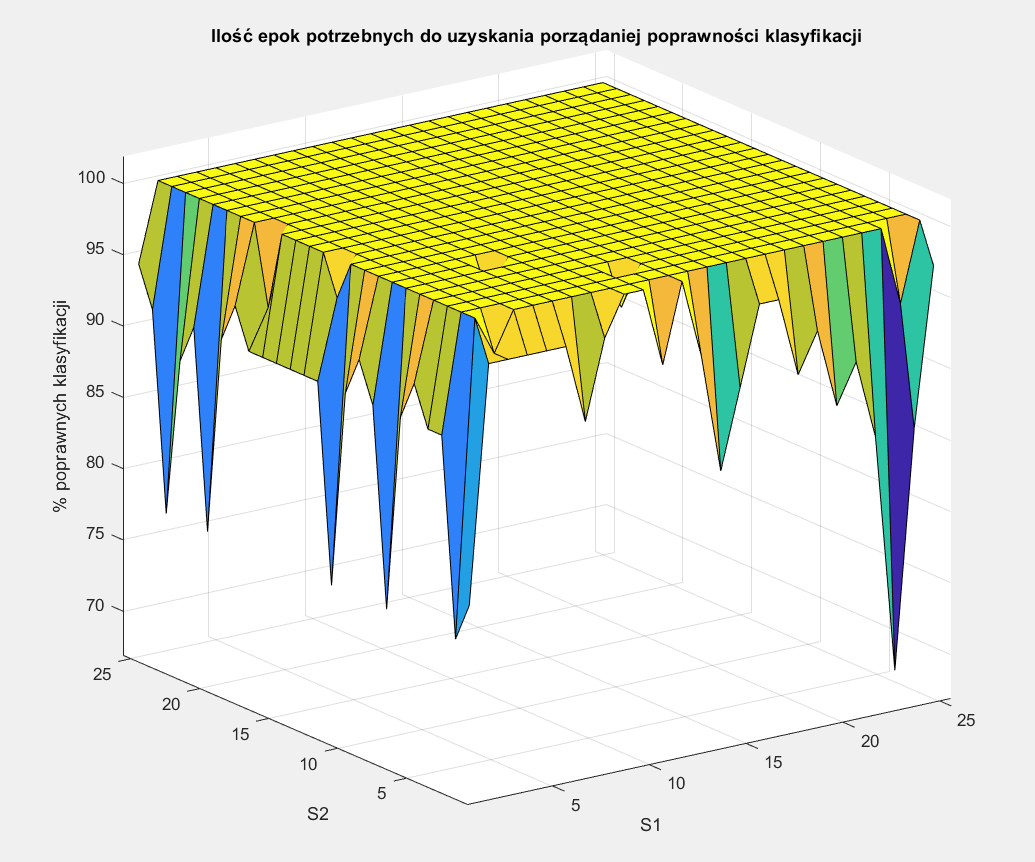
\includegraphics[width=13cm]{eks1_klas.png}
\caption{Wykres wypływu S1, S2 na poprawność klasyfikacji}
\end{figure}

Na wykresie \ref{eks1_klas} można zauważyć, że większość kombinacji liczby neuronów S1 i S2 proces uczenia zakończył się przed osiągnięciem maksymalnej ilości epok, co świadczy o tym, że przedstawiony zbiór danych jest niewymagający. W celu poprawnej analizy danych wykreślono powierzchnię funkcji minimalnej ilości epok potrzebnych do osiągnięcia zakładanego błędu uczenia SSE.
\clearpage
\begin{figure}[H]
\label{eks1_epochs}
\centering
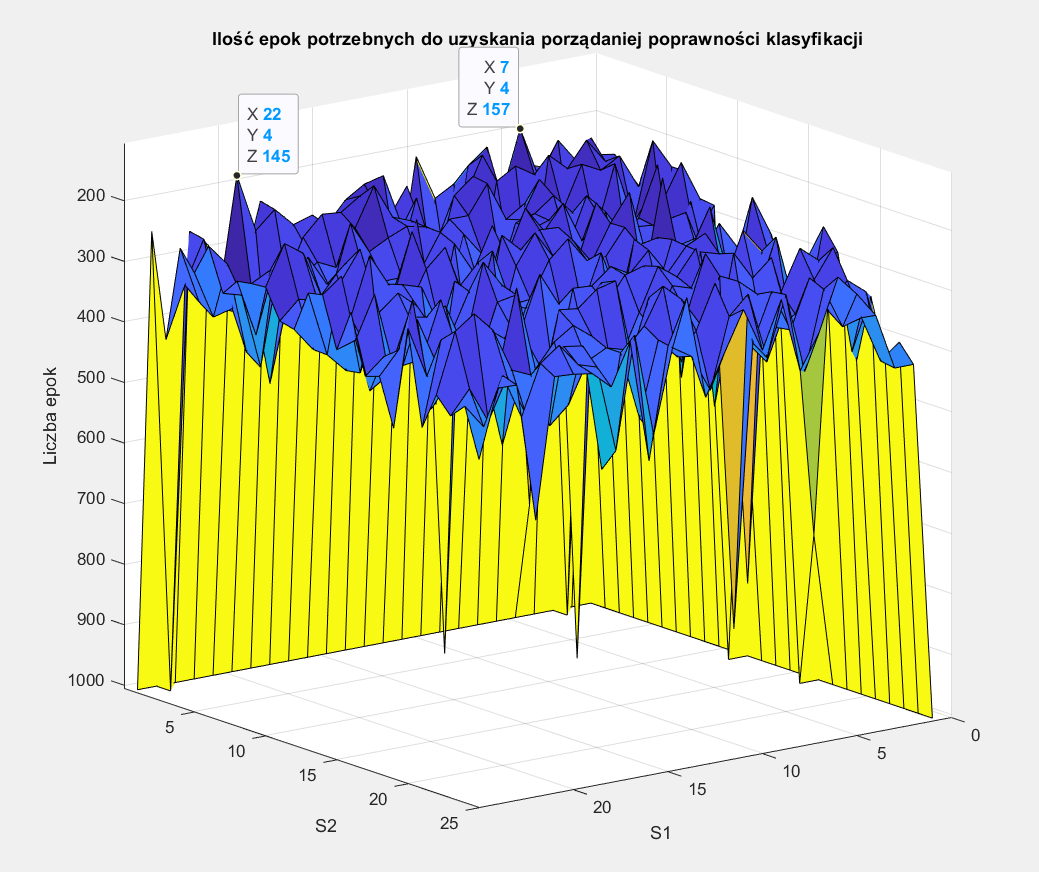
\includegraphics[width=13cm]{eks1_epochs.png}
\caption{Wykres wypływu S1, S2 na ilość epok potrzebnych do osiągnięcia zakładanego SSE}
\end{figure}

W wyniku tego eksperymentu okazało się, że dla większości kombinacji S1 i S2 sieć osiąga $100\%$ dokładności klasyfikacji. Skuteczność tą osiąga najszybciej dla kombinacji $<22,4>$, którą sieć osiągnęła po 145 epokach. Drugą parą jest kombinacja $<7,4>$, dla której zadaną skuteczność osiągnięto po 157 epokach.



\subsection{Eksperyment 2 - badanie parametrów $lr_{inc}$ oraz $lr_{dec}$}
Celem drugiego eksperymentu było wyznaczenie optymalnych wartości parametrów $lr_{inc}$ oraz $lr_{dec}$ odpowiedzialnych za modyfikację współczynnika uczenia na podstawie bieżącego błędu SSE. Na potrzeby eksperymentu przyjęto parametry uczenia określone w tabeli \ref{tab2}, zmianie poddane zostały parametry:
\begin{itemize}
\item learning rate accelerate - w przedziale $< 0.9; 1.9 >$, ze skokiem co 0.05
\item learning rate decelerate - w przedziale $< 0.1; 1.1 >$, ze skokiem co 0.05
\end{itemize}


\begin{lstlisting}[language=Python,caption=Algorytm realizujący eksperyment 2,label={eks2}]
import sys
import network
from data import loadData
import pandas as pd
import numpy as np
trainData, testData = loadData()
lr_inc_vec=np.arange(0.9,1.91,0.05)
lr_dec_vec=np.arange(0.1,1.11,0.05)
results = []
name=sys.argv[3]
name='inc_dec__'+name+'.csv'
for lr_inc in lr_inc_vec:
	for lr_dec in lr_dec_vec:
		result = [lr_inc,lr_dec]
		net = network.Network([13, int(sys.argv[1]), int(sys.argv[2]), 3])
		result.extend(net.train(trainData,testData,inc=lr_inc,dec=lr_dec))
		results.append(result)

results=pd.DataFrame(results)
results.to_csv(name,index=None,header=None)


\end{lstlisting}


\subsubsection{Badania dla $S1=22$, $S2=4$}

\begin{figure}[H]
\centering
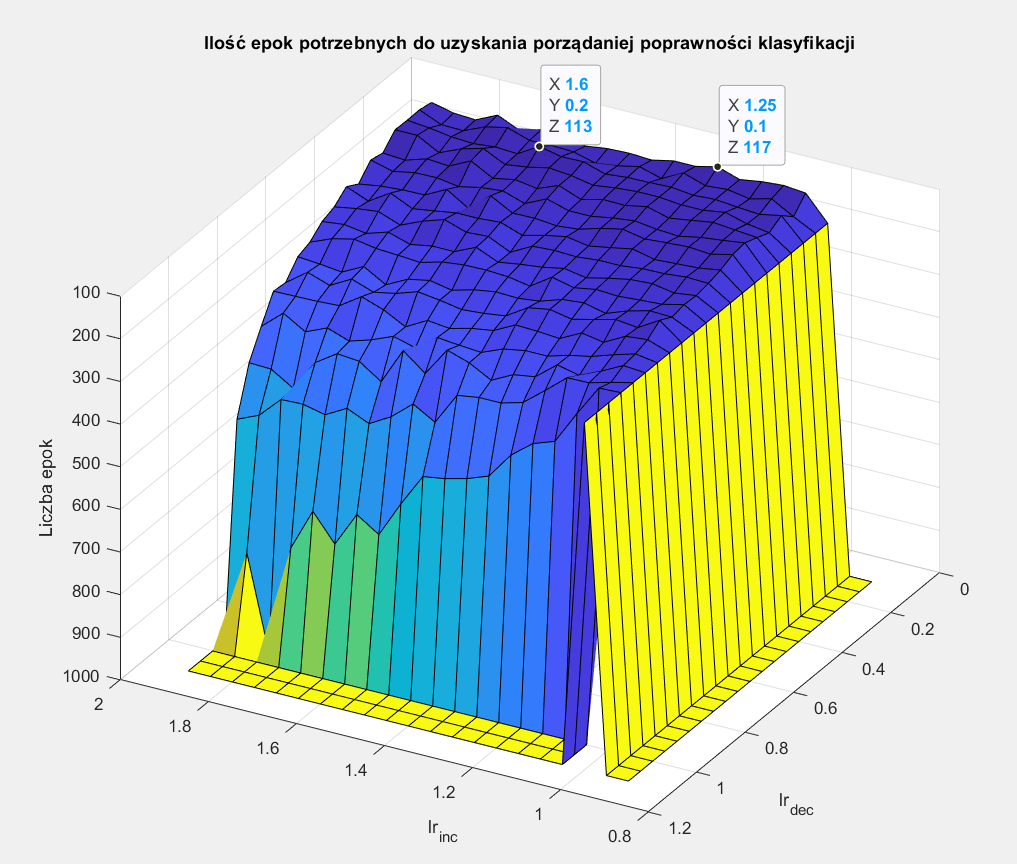
\includegraphics[width=13cm]{eks2_1.png}
\caption{Zależność poprawności klasyfikacji od $lr_{inc}$ oraz $lr_{dec}$ dla $S1=22$, $S2=4$}
\label{eks2_1}
\end{figure}


Rysunek \ref{eks2_1} przedstawia powierzchnię funkcji ilości epok potrzebnej do osiągnięcia zamierzonego błędu w zależności od wartości parametru learning rate accelerate oraz learning rate decelerate. Dla S1= 22, S2 = 4 największą poprawność uczenia osiągnięto dla wartości $lr_{inc}  =  1.6$, oraz $lr_{dec} = 0.2$. Natomiast najgorszy wynik uzyskano gdy $lr_{inc}$ wynosił 0.9 lub $lr_{dec}$ był większy niż 1.

\subsubsection{Badania dla $S1=7$, $S2=4$}

\begin{figure}[H]
\centering
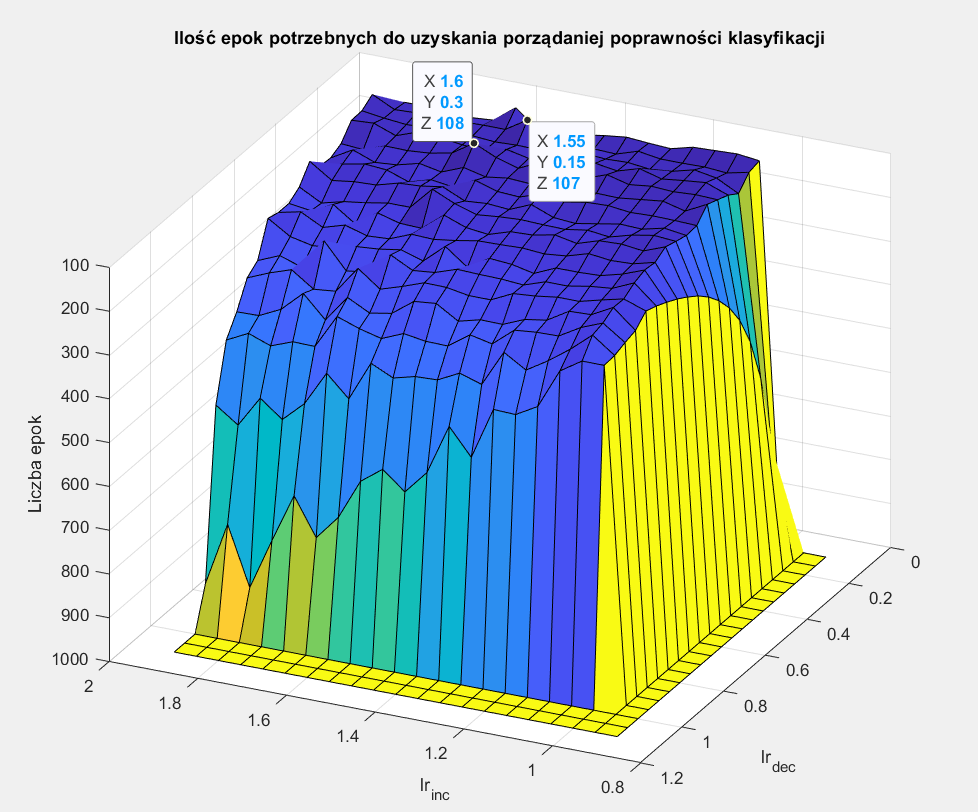
\includegraphics[width=13cm]{eks2_2.png}
\caption{Zależność poprawności klasyfikacji od $lr_{inc}$ oraz $lr_{dec}$ dla $S1=7$, $S2=4$}
\label{eks2_2}
\end{figure}

Rysunek \ref{eks2_2} przedstawia powierzchnię funkcji ilości epok potrzebnej do osiągnięcia zamierzonego błędu w zależności od wartości parametru learning rate accelerate oraz learning rate decelerate. Dla S1= 7, S2 = 4 największą poprawność uczenia osiągnięto dla wartości $lr_{inc}  =  1.55$, oraz $lr_{dec} = 0.15$. Natomiast najgorszy wynik uzyskano gdy $lr_{inc}$ wynosił 0.9 lub $lr_{dec}$ był większy niż 1.

Porównując przedstawione wyżej wykresy i wartości, można wywnioskować, że sieć w parametrach S1= 7, S2 = 4 jest lepiej uwarunkowana dla badanego zestawu danych. 


\subsection{Eksperyment 3 - badanie parametru er}
Celem trzeciego eksperymentu było zbadanie wpływu współczynnika maksymalnego przyrostu błędu $er$ na ilość potrzebnych epok do osiągnięcia zakładanej wartości błędu SSE. Domyślnie parametr ten wynosił $1.04$. Na potrzeby eksperymentu zmieniano wartość $er$ w zakresie $[1.01; 1.09]$. Badania przeprowadzono dla maksymalnej liczby 1000 epok, $lr_{inc}  = 1.55$, $lr_{dec} = 0.15$ oraz $lr_{inc}  = 1.6$, $lr_{dec} = 0.3$ dla parametrów S1 = 7, S2 = 4. Listing \ref{eks3} przedstawia kod, którego użyto do eksperymentu.

\begin{lstlisting}[language=Python,caption=Algorytm realizujący eksperyment 3,label={eks3}]
import sys
import network
from data import loadData
import pandas as pd
import numpy as np
trainData, testData = loadData()
err_inc_vec=np.arange(1.01,1.091,0.01)
results = []
name=sys.argv[3]
name='err_inc'+name+'.csv'
for err in err_inc_vec:
	result = [err]
	net = network.Network([13, 7, 4, 3])
	result.extend(net.train(trainData,testData,inc=float(sys.argv[1]),dec=float(sys.argv[2]),err_inc=err))
	results.append(result)

results=pd.DataFrame(results)
results.to_csv(name,index=None,header=None)

\end{lstlisting}

\begin{figure}[H]
\centering
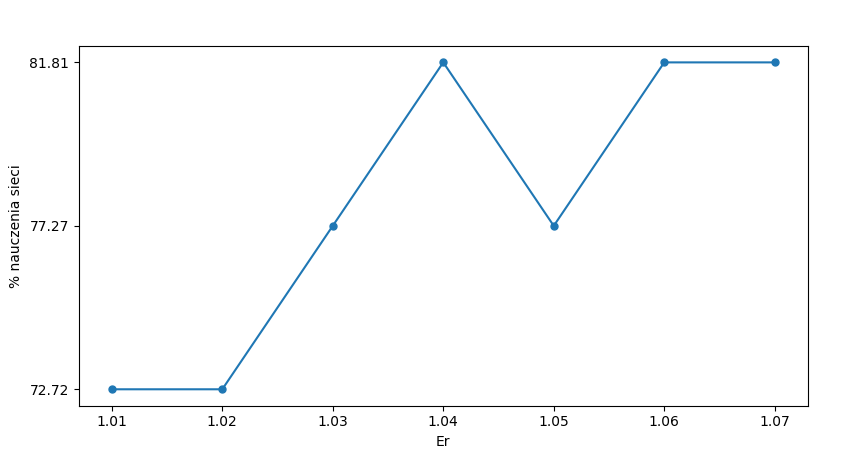
\includegraphics[width=12cm]{eks3.png}
\caption{Wykres wpływu parametru er na poprawność klasyfikacji}
\label{ryseks3}
\end{figure}

Rysunek \ref{ryseks3} obrazuje wyniki wykonanego badania.
Na jego podstawie można ocenić, że dla pierwszej kombinacji optymalną wartością parametru $er$ jest wartość z przedziału $<1.03;1.06>$, natomiast dla drugiej pary jest to przedział $<1.04;1.05>$.


\subsection{Eksperyment 4 - badanie wielkości podzbiorów}
Celem czwartego eksperymentu było wyznaczenie optymalnej wielkości mini-batcha, dla którego obliczany jest gradient. Jako parametry przyjęto najoptymalniejsze z poprzednich eksperymentów: $S1 = 7; S2=4; lr_{inc}=1.55; lr_{dec}=0.15; err_inc=1.04$. Rozmiar mini-batchy został określony według następującego wzoru $len(trainingData)\over{n}$, gdzie $n$ należy do przedziału $<1; 50>$ ze skokiem co 1.

\begin{lstlisting}[language=Python,caption=Algorytm realizujący eksperyment 3,label={eks4}]
	import network
	from data import loadData
	import pandas as pd
	import numpy as np
	from tabulate import tabulate
	trainData, testData = loadData()
	results = []
	n=len(trainData)
	size_vec = [n//x for x in range(1,50)]
	for size in size_vec:
	result = [size]
	net = network.Network([13, 7, 4, 3])
	result.extend(net.train(trainData,testData,inc=1.55,dec=0.15,err_inc=1.04,mini_batch_size=size))
	results.append(result)
	
	results=pd.DataFrame(results)
	results.to_csv('batch.csv',index=None,header=None)
	
	
\end{lstlisting}

\begin{figure}[H]
	\centering
	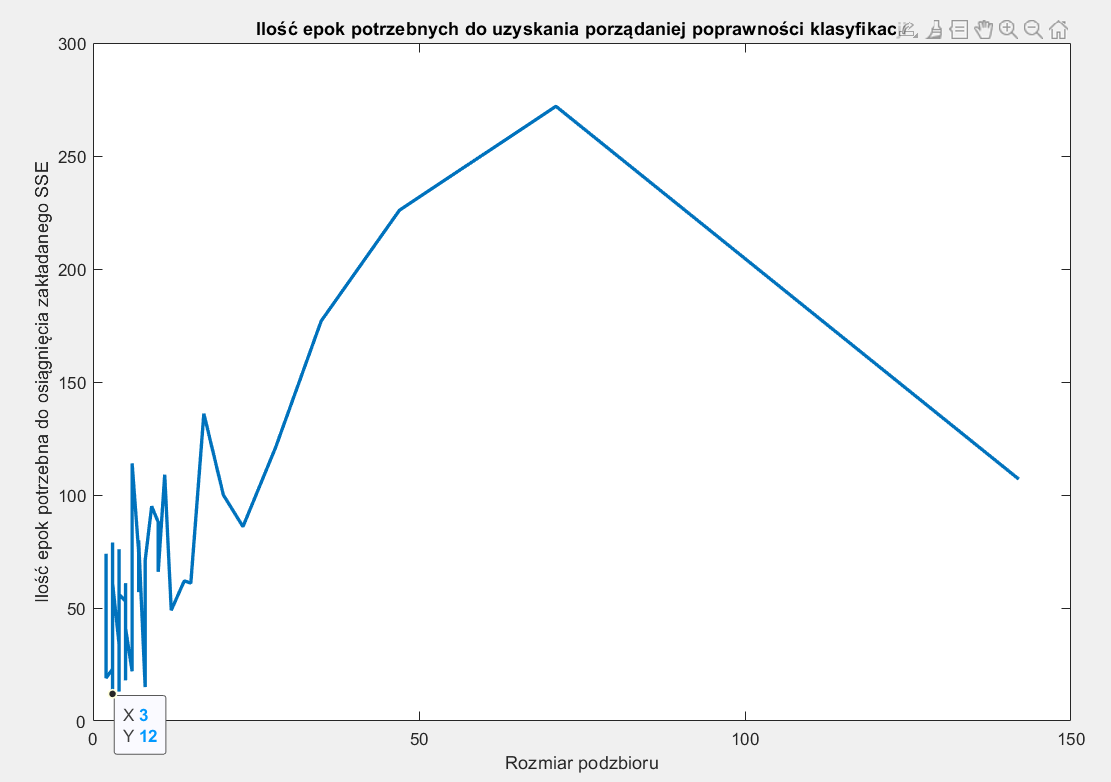
\includegraphics[width=15cm]{eks4.png}
	\caption{Wykres wpływu parametru $mini\_batch\_size$ na poprawność klasyfikacji}
	\label{ryseks4}
\end{figure}

Z wykresu \ref{ryseks4} można zauważyć, że prędkość uczenia wzrasta wraz ze spadkiem rozmiaru pojedynczego podzbioru. Najbardziej optymalną wartością tego parametru jest wartość 3, dla której sieć potrzebuje tylko 12 epok do osiągnięcia zamierzonej wartości SSE. 


\clearpage
\section{Podsumowanie i wnioski końcowe}

Cel projektu, tj. zrealizowanie sztucznej sieci neuronowej uczonej algorytmem wstecznej propagacji błędu z przyśpieszeniem metodą adaptacyjnego współczynnika uczenia (trainbpa) uczącej się diagnozowania choroby został zrealizowany. Użyto w tym celu własnej implementacji sieci neuronowej napisanej w jęyku Python na podstawie książki Michaela Nielsena \cite{nielsen}. 

Zadany zbiór okazał się być zbiorem niewymagającym. Dla znacznej większości kombinacji parametrów S1 oraz S2 sieć osiągała $100\%$ poprawność klasyfikacji. 

Eksperymenty pozwoliły na określenie optymalnych wartości parametrów umożliwiających jak najszybsze uczenie się sieci. 

Pierwszy eksperyment polegał na dostosowaniu ilości neuronów w warstwie I i II. Minimalną ilość epok potrzebnych do nauczenia sieci osiągnięto dla zestawu $\{22,4\}$ oraz $\{7,4\}$. 

Celem drugiego eksperymentu było wyznaczenie optymalnych wartości parametrów $lr_{inc}$ oraz $lr_{dec}$. Badanie to przeprowadzono dla najlepszych wyników otrzymanych z eksperymentu 1. Na podstawie uzyskanych wykresów można także wywnioskować, że sieć jest lepiej uwarunkowana dla $S1 = 7$ oraz $S2 = 4$.

Trzeci, ostatni eksperyment przeprowadzono w celu wyznaczenia najbardziej optymalnego parametru $er$. Obserwując wynik badania, można zauważyć, że sieć osiąga najlepsze wartości dla $er = \{1.04, 1.06, 1.07\}$. 

Przeprowadzone eksperymenty pozwoliły na ustalenie optymalnych wartości parametrów, dla których sieć osiągała najlepszy wynik poprawności klasyfikacji. Badania te wykazały, że domyślne parametry z programu Matlab są najkorzystniejsze. 

\clearpage


\addcontentsline{toc}{section}{Literatura}

\begin{thebibliography}{4}
\bibitem{dane} UCI Machine Learning Repository\\https://archive.ics.uci.edu/ml/datasets/Wine [Dostęp 14.05.2022 r.]
\bibitem{nielsen} Michael A. Nielsen, "Neural Networks and Deep Learning", Determination Press, 2015
\bibitem{norm} http://sztuczna-inteligencja.eprace.edu.pl/1001,Funkcje-normalizacji.html [Dostęp 14.05.2022 r.]
\bibitem{zajdel2}dr hab. inż. Roman Zajdel prof. PRz, PRz, KIiA, Sztuczna inteligencja, Laboratorium, Ćw8 Sieć jednokierunkowa jednowarstwowa\\
http://materialy.prz-rzeszow.pl/pracownik/pliki/34/sztuczna-inteligencja-cw8-siec-jednowarstw.pdf [Dostęp 09.06.2022 r.]
\bibitem{zajdel1}dr hab. inż. Roman Zajdel prof. PRz, PRz, KIiA, Sztuczna inteligencja, Laboratorium, Ćw9 Sieć jednokierunkowa wielowarstwowa\\
http://materialy.prz-rzeszow.pl/pracownik/pliki/34/sztuczna-inteligencja-cw9-siec-wielowarstw.pdf [Dostęp 09.06.2022 r.]
\bibitem{mamczur}https://miroslawmamczur.pl/czym-jest-i-jak-sie-uczy-sztuczna-siec-neuronowa/ [Dostęp 21.05.2022 r.]
\bibitem{leksykon} R. Tadeusiewicz, M. Szaleniec „Leksykon sieci neuronowych”, Wrocław 2015
\bibitem{github} Repozytorium z własną implementacją sieci neuronowej\\ https://github.com/saimon833/ai\_project [Dostęp 10.06.2022 r.]


\end{thebibliography}

\clearpage


\end{document} 
